\documentclass[a4paper]{article}

\usepackage[per-mode=symbol,separate-uncertainty=true]{siunitx}
\usepackage{amsmath}
\usepackage{float}
\usepackage{graphicx}
\usepackage[a4paper,top=3cm,bottom=2cm,left=3cm,right=3cm,marginparwidth=1.75cm]{geometry}
\usepackage{mathtools}
\usepackage{subcaption}
\usepackage{xcolor}
\usepackage{xspace}
\usepackage{fancyhdr}

\newcommand{\inv}{\texttt{INV\_X4}\xspace}
\newcommand{\ha}{\texttt{HA\_X1}\xspace}

\title{Digital Microelectronics 2018 \\ Final project report}
\author{Marco Andorno (247222)\\ Michele Caon (253027) \\ Matteo Perotti (251453)}

\begin{document}

% INTRO
\begin{center}

\thispagestyle{empty}

\textbf{\Large Digital Microelectronics}\\[1.0cm]
\textsc{\Large Politecnico di Torino}\\[0.5cm]
\textsc{\large Dipartimento di Elettronica e Telecomunicazioni}\\[1cm]

% TITLE
\huge \textbf{Final Project: \\ Standard Cell layout of an inverter and a half-adder}

\end{center}

% AUTHORS
\vfill
\large
\begin{flushleft}
\makeatletter
\emph{Group 5:}\\
\@author \\
\vspace{1cm}
\normalsize Date: \today
\makeatother
\end{flushleft}

%\maketitle

\newpage

\pagestyle{fancy}
\lhead{}
\chead{}
\rhead{\leftmark}
\lfoot{\thepage}
\cfoot{}
\rfoot{}
\renewcommand{\headrulewidth}{0.3pt}
\renewcommand{\footrulewidth}{0.3pt}

% \tableofcontents
% \newpage

\section{Introduction}
The goal of this final project is to design and characterize two logic gates of a standard cell library. These are in particular an inverter whose transistors have width four times the minimum (\inv in the following), and a half adder (\ha in the following).

The design starts with the schematic drawing, using an available \texttt{.png} image as a reference, which has to be simulated as an initial condition. Then, the layout of the cell must be drawn and the parasitic elements must be extracted from it. Finally, those parasitics must be used for the final characterization in order to fill in the Liberty file of the standard cell library.

\section{Inverter}
\subsection{Schematic}
Starting from the schematic of the available \texttt{.png} (figure \ref{fig:inv_png}), we copied it using Virtuoso Schematic Editor, obtaining the result shown in figure \ref{fig:inv_schematic}. Note that the four PMOS and NMOS transistors in parallel will be just one large transistor in the layout.
\begin{figure}[H]
	\centering
	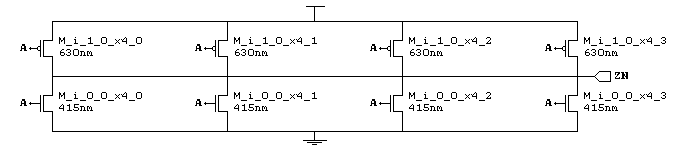
\includegraphics[width=1.2\linewidth]{../INV_X4/INV_X4.png}
	\caption{Reference schematic of the inverter}
	\label{fig:inv_png}
\end{figure}
\begin{figure}[H]
	\centering
	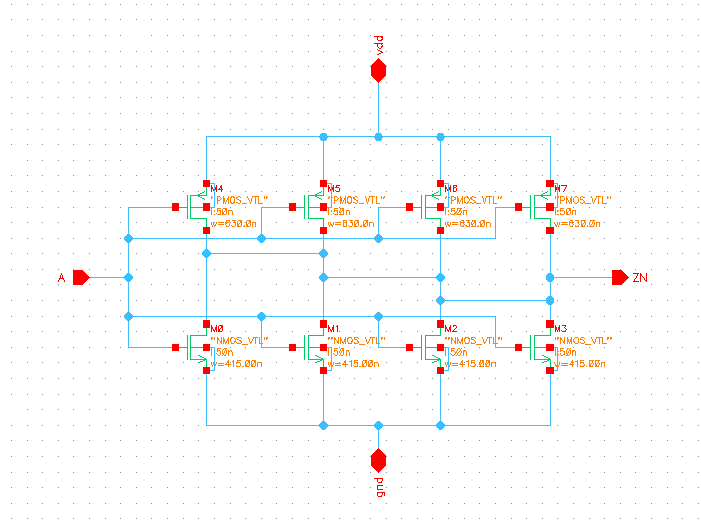
\includegraphics[width=\linewidth]{../INV_X4/INV_X4_schematic.png}
	\caption{Final schematic of \inv}
	\label{fig:inv_schematic}
\end{figure}

We then carried out some preliminary simulations using a test bench, to confirm that the circuit works correctly. We measured rise and fall times, as well as propagation delays, that will be compared with the actual characterization later on. We also measured the transfer characteristic, shown in figure \ref{fig:inv_tchar}.
\begin{figure}[H]
	\centering
	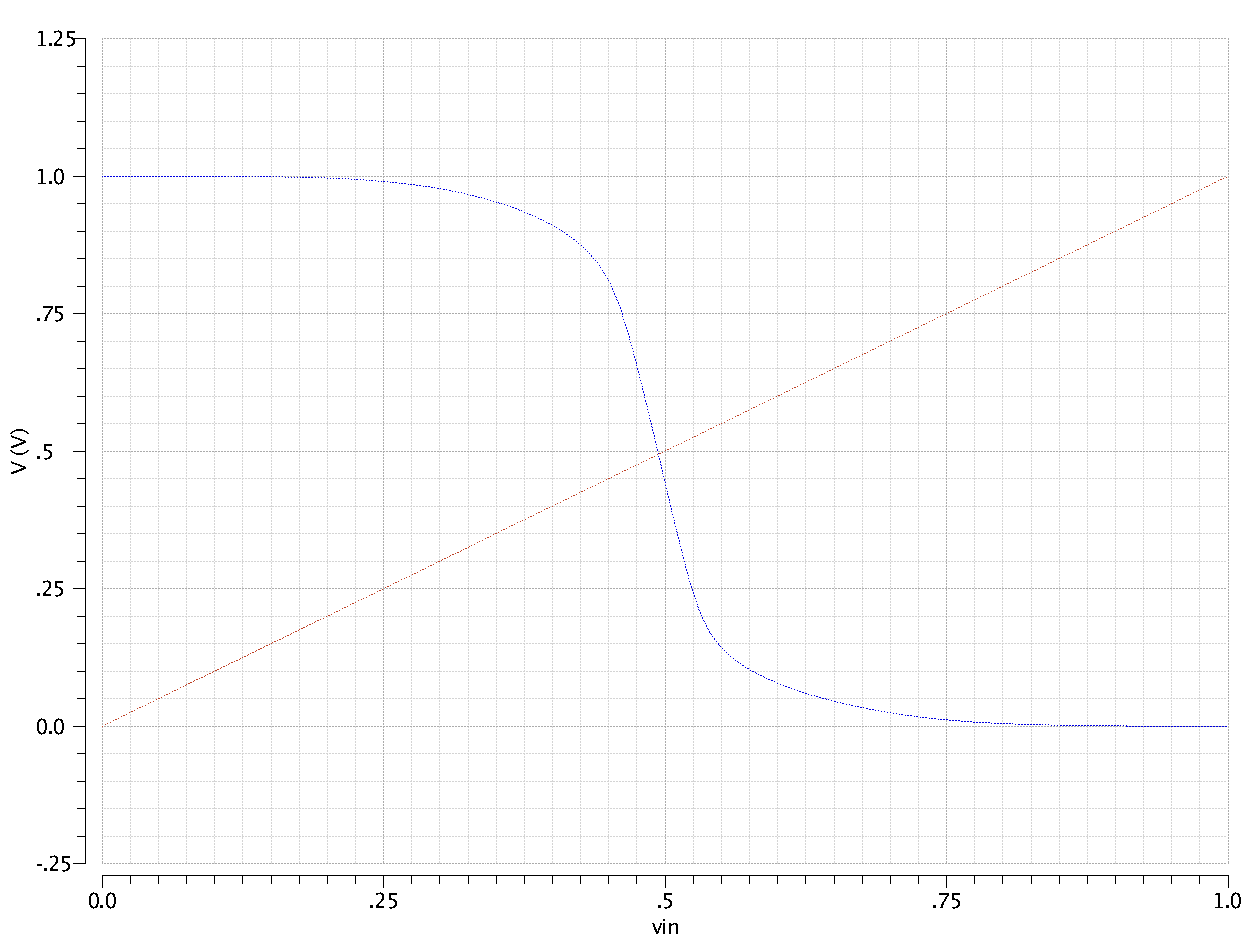
\includegraphics[width=.7\linewidth]{../INV_X4/INV_X4_transfer_char.pdf}
	\caption{Inverter transfer characteristic}
	\label{fig:inv_tchar}
\end{figure}


\subsection{Layout}
\subsection{Characterization}

\section{Half adder}
\subsection{Schematic}
The schematic was drawn using Virtuoso schematic editor.

\begin{figure}[H]
      \centering
       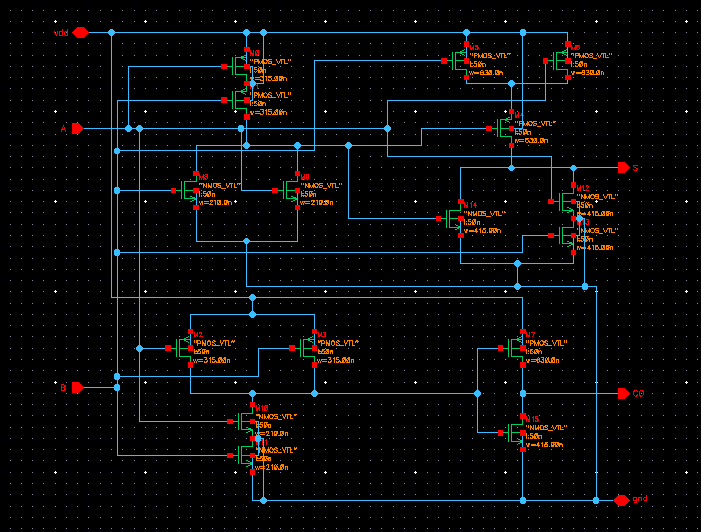
\includegraphics[width=12cm]{./Images/HA/HAX1_schematic.png}
\caption{HAX1 schematic}
\label{fig: HAX1_sch}
\end{figure}

\subsection{Layout}
Given that the layout of the half adder is quite more complex than the one of the inverter, we started by deeply analyzing the possible approaches using the pen-and-paper method. The final solution that we found consisted in sharing source/drain diffusions as much as possible, in order to minimize the area in the horizontal direction.

When actually drawing the design in Virtuoso, we made sure of running the Design Rule Checker very often, in order to avoid problems in advance.

Layout design started looking at the schematic. First of all we tried to put the two outputs on the opposite sides of the cell, because this way, if the input are brought over it in the middle with the \texttt{metal 2} and linked with vias, the input-output paths are more probably balanced in length. 
Thus we started drawing on a paper the first nMos of the inverter whose output was CO. With a view to share the sources/drains as much as possible we began putting all the transistors one near the other drawing only the strictly necessary metal.
We used different colours to have an easier readability and go on drawing only the \texttt{metal} for the sources/drains and the \texttt{polysilicon} for the gates until the end of the port and left the routing last. Then we completed the layout linking together the various elements coherently with the schematic view.

\begin{figure}[H]
      \centering
       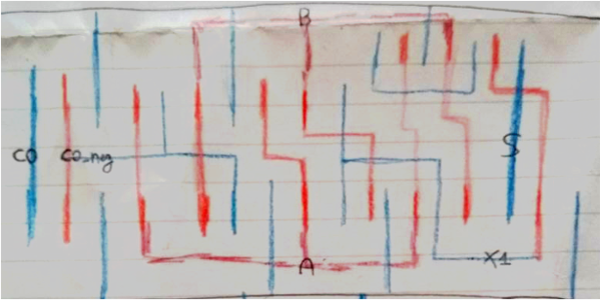
\includegraphics[width=12cm]{./Images/HA/layout_drw.png}
\caption{First sketch of the layout. Blue: metal1, red: polysilicon. Labels are not related with the position of the corresponding via.}
\label{fig: lay_drw}
\end{figure}

Then we converted this sketch in a real layout design using the Virtuoso embedded layout editor. During our sessions we paid attention to reduce every distance to the minimum with the aid of the meter tool and in accordance with the Design Rules. We made a lot of effort to have a cell with the minimum area because the area is directly linked to the yield of the process and to logic ports density, capacitance and therefore delay and power cost per commutation. The less is the area, the more ports can stay in a chip or the more the chip will be small, and it is harder to find defects on a single chip if it is small, because the density of the defects per unit area is about constant (higher yield for the process). The delay and the power costs rise with the area because if more material is used, more resistance/capacitance is added. For this reason we also tried to reduce the length of every wire.

The height of the cell is fixed because this is a standard cell. The top and the ground of it are made of metal which has to feed the transistors. Many entity like this one can be put one next to the other to form a line of cells packed together and fed with global Val-GND voltages. This way it is simpler to reach every port with its supply.

When we drew the layout with the editor we changed a little bit the connections. Instead of putting a single wire of \texttt{polysilicon} to connect each gate with the related input A/B, we used vias and \texttt{metal1}. It would have been interesting to compare the performances of two implementations.

\begin{figure}[H]
      \centering
       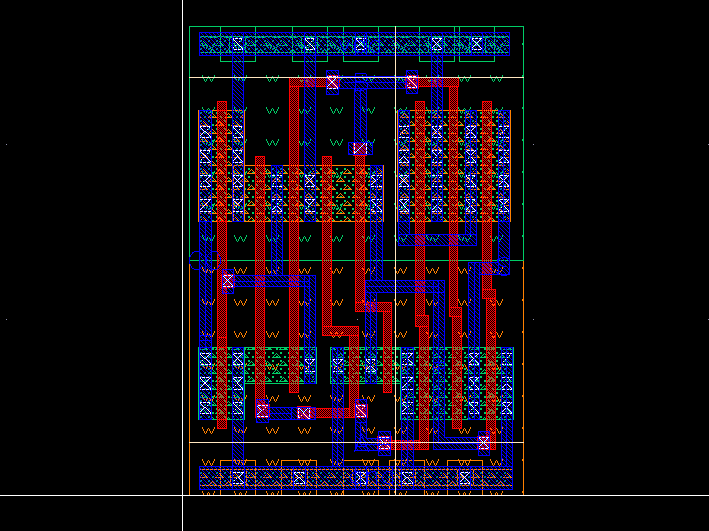
\includegraphics[width=12cm]{./Images/HA/HAX1_poly-metal_layout.png}
\caption{HAX1 layout, more metal1 and vias on pull-down connections}
\label{fig: HAX1_lay_drw}
\end{figure}

In the pull up network the advantage of putting \texttt{metal1} seems to be huge, whereas in the pull down network it's not so clear. We present here another possible implementation. For time reasons we have characterized only the first one, though.

\begin{figure}[H]
      \centering
       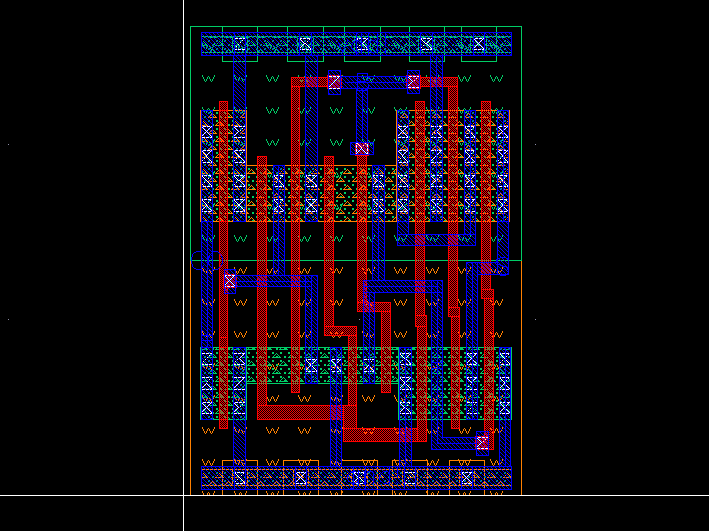
\includegraphics[width=12cm]{./Images/HA/HAX1_poly_layout.png}
\caption{HAX1 layout, more polysilicon on pull-down connections}
\label{fig: HAX1_layPoly_drw}
\end{figure}

\subsection{Characterization}



\end{document}
